\chapter{Flores, frutos e sementes}\label{ch:g3:flowers-fruits-seeds}

Em abril a cerejeira fica branca de \omterm{def:g3:flowers-fruits-seeds:parts}{flores}; em junho ela fica
carregada de cerejas. Para onde foram as \omterm{def:g3:flowers-fruits-seeds:parts}{flores} --- e de onde vieram
os \omterm{prop:g3:flowers-fruits-seeds:transform}{frutos}? A resposta é uma das transformações mais bonitas do mundo
vivo: a \omterm{def:g3:flowers-fruits-seeds:parts}{flor} não some, ela \emph{vira} o \omterm{prop:g3:flowers-fruits-seeds:transform}{fruto}.

\section{Olhando dentro de uma flor}

\begin{definition}[As partes de uma flor]\label{def:g3:flowers-fruits-seeds:parts}
A \emph{flor}\index{flor} é a parte da \omterm{def:g1:plants-around-us:plant}{planta} que vai fazer as
\omterm{prop:g3:flowers-fruits-seeds:transform}{sementes}. De fora para dentro:
\begin{enumerate}
  \item as \emph{pétalas}\index{pétala}, coloridas e perfumadas, que
        atraem os \omterm{prop:g3:sorting-living-things:groups}{insetos} visitantes;
  \item os \emph{estames}\index{estame}, hastes finas polvilhadas de
        \emph{pólen}\index{pólen}, um pó amarelo bem fininho;
  \item bem no meio, o \emph{pistilo}\index{pistilo}, um frasquinho;
        lá no fundo dele ficam as futuras \omterm{prop:g3:flowers-fruits-seeds:transform}{sementes} da flor.
\end{enumerate}
\end{definition}

\begin{omfigure}
\begin{tikzpicture}
  \node[anchor=south west, inner sep=0] (img) at (0,0)
    {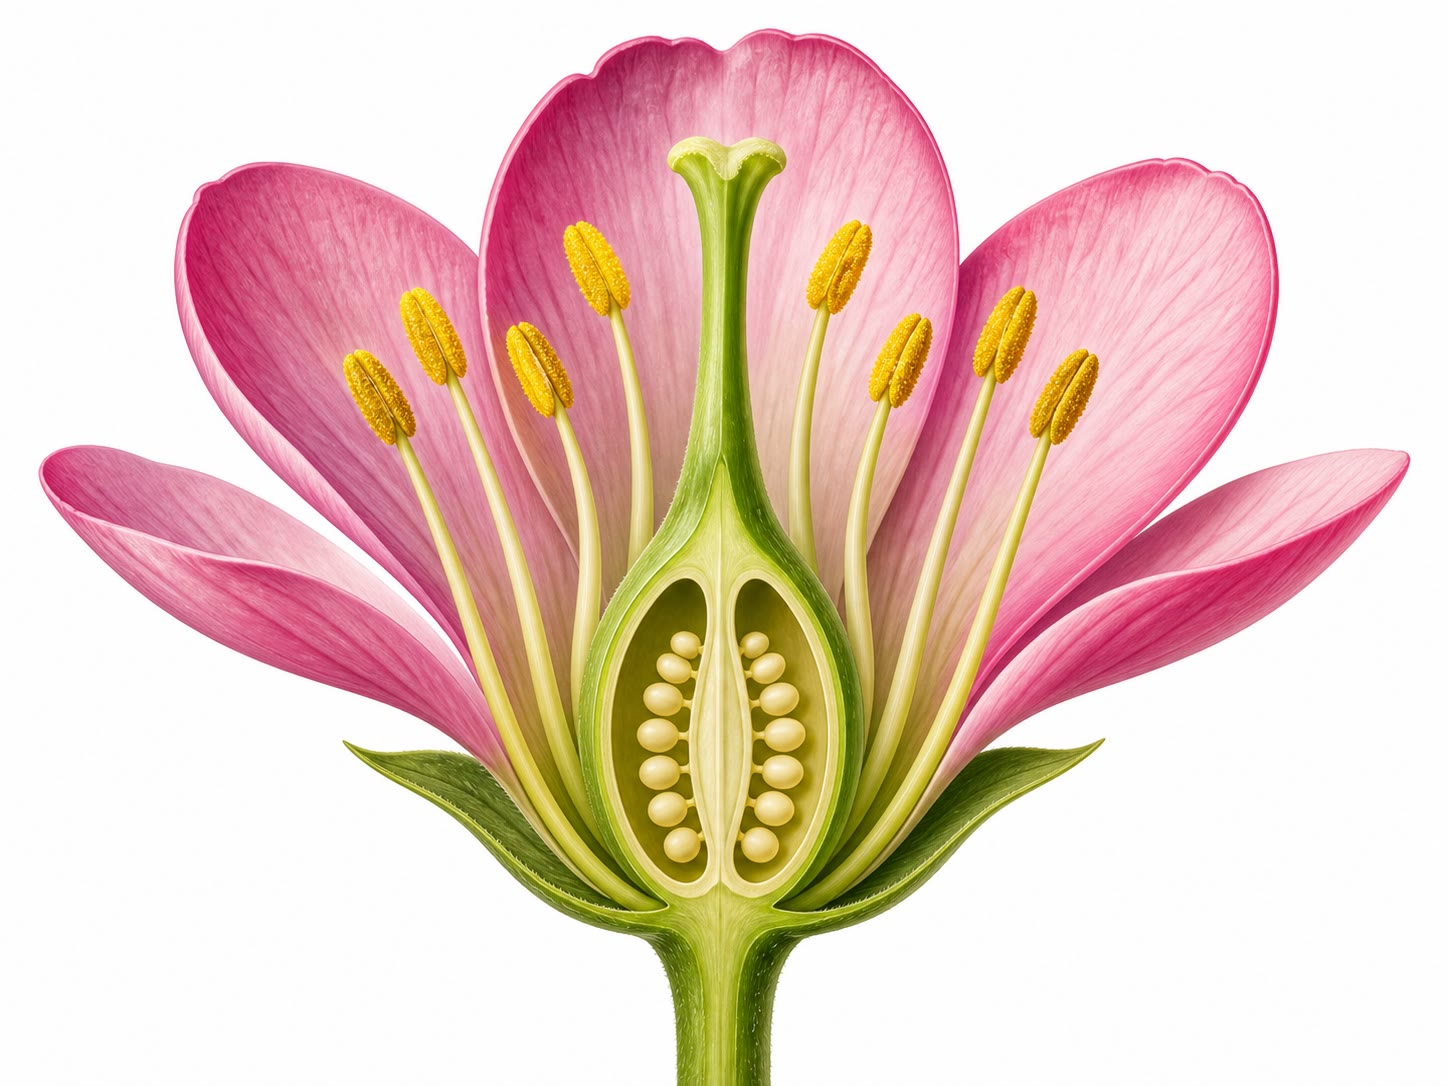
\includegraphics[width=0.6\linewidth]{images/book1/ai/fig-flower-cutaway.jpg}};
  \begin{scope}[x={(img.south east)}, y={(img.north west)},
      every node/.style={font=\small}]
    \draw[omDef, thick] (0.82,0.80) -- (0.93,0.90) node[above] {pétala};
    \draw[omDef, thick] (0.72,0.68) -- (1.03,0.66)
      node[right, align=left] {estame, polvilhado\\ de pólen};
    \draw[omDef, thick] (0.56,0.36) -- (1.03,0.34)
      node[right, align=left] {pistilo: as futuras\\ sementes estão dentro};
    \draw[omDef, thick] (0.505,0.05) -- (0.66,0.04) node[right] {caule};
  \end{scope}
\end{tikzpicture}

{\small Dentro de uma \omterm{def:g3:flowers-fruits-seeds:parts}{flor} cortada ao meio: as \omterm{def:g3:flowers-fruits-seeds:parts}{pétalas} em volta, os
\omterm{def:g3:flowers-fruits-seeds:parts}{estames} carregados de \omterm{def:g3:flowers-fruits-seeds:parts}{pólen} e o \omterm{def:g3:flowers-fruits-seeds:parts}{pistilo} no centro, com as futuras
\omterm{prop:g3:flowers-fruits-seeds:transform}{sementes} lá dentro.}
\end{omfigure}

\begin{example}[Dissecando uma tulipa]\label{ex:g3:flowers-fruits-seeds:tulip}
Abra com cuidado uma tulipa que está murchando, \omterm{def:g3:flowers-fruits-seeds:parts}{pétala} por \omterm{def:g3:flowers-fruits-seeds:parts}{pétala}.
Lá dentro estão os \omterm{def:g3:flowers-fruits-seeds:parts}{estames} --- passe um deles no dedo e ele deixa um
pó amarelo de \omterm{def:g3:flowers-fruits-seeds:parts}{pólen} --- e, no meio, o \omterm{def:g3:flowers-fruits-seeds:parts}{pistilo} verde e gordinho.
Corte o \omterm{def:g3:flowers-fruits-seeds:parts}{pistilo} de través (com a faca nas mãos de um adulto) e lá
estão elas: fileiras de futuras \omterm{prop:g3:flowers-fruits-seeds:transform}{sementes} claras e minúsculas.
\end{example}

\section{Da flor ao fruto}

\begin{proposition}[Polinização e depois transformação]\label{prop:g3:flowers-fruits-seeds:transform}
Para a transformação começar, o \omterm{def:g3:flowers-fruits-seeds:parts}{pólen} precisa chegar ao \omterm{def:g3:flowers-fruits-seeds:parts}{pistilo} ---
esse passo é a \emph{polinização}\index{polinização}. As abelhas e
outros \omterm{prop:g3:sorting-living-things:groups}{insetos} fazem quase todo o transporte, polvilhados de \omterm{def:g3:flowers-fruits-seeds:parts}{pólen}
enquanto bebem de \omterm{def:g3:flowers-fruits-seeds:parts}{flor} em \omterm{def:g3:flowers-fruits-seeds:parts}{flor}; o vento também faz um pouco. Depois
da polinização:
\begin{itemize}
  \item as \omterm{def:g3:flowers-fruits-seeds:parts}{pétalas} e os \omterm{def:g3:flowers-fruits-seeds:parts}{estames}, com o trabalho feito, murcham e caem;
  \item o \omterm{def:g3:flowers-fruits-seeds:parts}{pistilo} incha e vira o \emph{fruto}\index{fruto};
  \item as futuras \omterm{prop:g3:flowers-fruits-seeds:transform}{sementes} que estão dentro dele viram as
        \emph{sementes}\index{semente}.
\end{itemize}
Um \omterm{prop:g3:flowers-fruits-seeds:transform}{fruto} é um \omterm{def:g3:flowers-fruits-seeds:parts}{pistilo} transformado, e todo \omterm{prop:g3:flowers-fruits-seeds:transform}{fruto} de verdade carrega
\omterm{prop:g3:flowers-fruits-seeds:transform}{sementes}.
\end{proposition}
\admitted

\begin{example}[Acompanhando uma cereja acontecer]\label{ex:g3:flowers-fruits-seeds:cherry}
Siga uma única \omterm{def:g3:flowers-fruits-seeds:parts}{flor} de cerejeira. Abril: \omterm{def:g3:flowers-fruits-seeds:parts}{pétalas} brancas, abelhas
zumbindo. Maio: as \omterm{def:g3:flowers-fruits-seeds:parts}{pétalas} caem como neve; onde estava cada \omterm{def:g3:flowers-fruits-seeds:parts}{flor},
uma bolinha verde --- o \omterm{def:g3:flowers-fruits-seeds:parts}{pistilo} inchando. Junho: a bolinha ficou
vermelha e doce --- uma cereja, com o caroço (a \omterm{def:g2:from-seed-to-plant:seed}{semente} dela)
dentro. A \omterm{def:g3:flowers-fruits-seeds:parts}{flor} não caiu; só as \omterm{def:g3:flowers-fruits-seeds:parts}{pétalas} dela caíram.
\end{example}

\begin{remark}[Sem abelhas, sem cerejas]\label{rem:g3:flowers-fruits-seeds:bees}
Quem cultiva cerejeiras recebe de bom grado as colmeias dos
apicultores no pomar --- sem as visitas dos \omterm{prop:g3:sorting-living-things:groups}{insetos}, a maioria das
\omterm{def:g3:flowers-fruits-seeds:parts}{flores} ficaria sem polinização e cairia sem nunca virar \omterm{prop:g3:flowers-fruits-seeds:transform}{fruto}. A
abelha não está roubando da \omterm{def:g3:flowers-fruits-seeds:parts}{flor}; a \omterm{def:g3:flowers-fruits-seeds:parts}{flor} e a abelha se alimentam uma
à outra: néctar para a abelha, entrega de \omterm{def:g3:flowers-fruits-seeds:parts}{pólen} para a \omterm{def:g1:plants-around-us:plant}{planta}.
\end{remark}

\begin{omfigure}
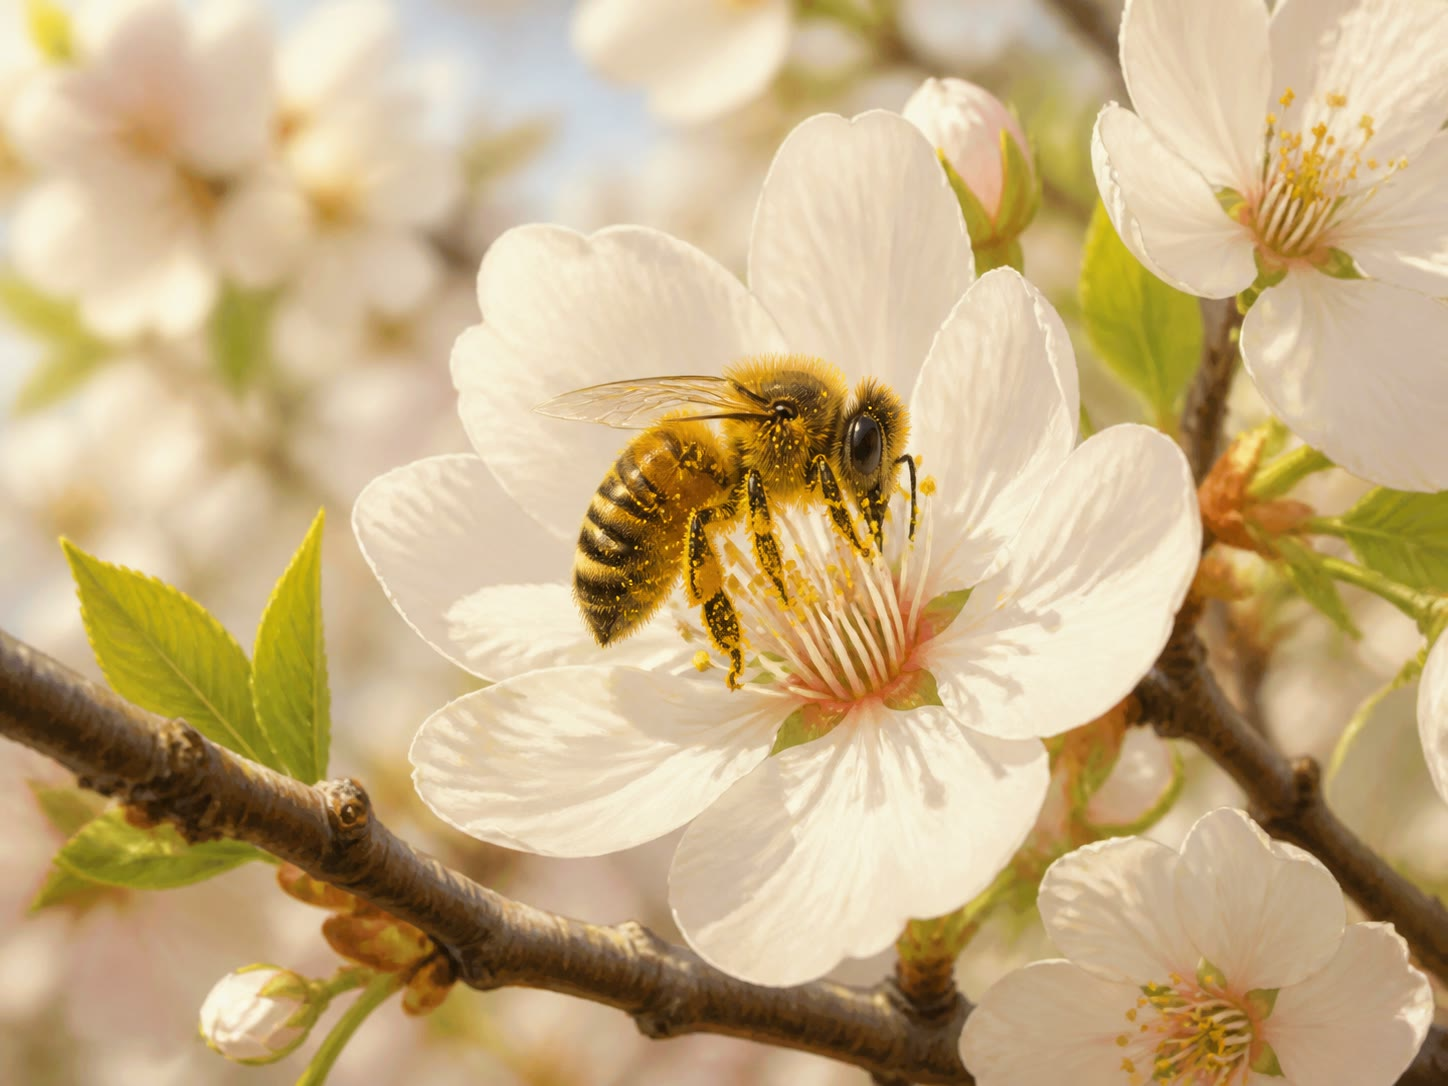
\includegraphics[width=0.58\linewidth]{images/book1/ai/g3-flowers-bee.jpg}

{\small Polinização em andamento: uma abelha no fundo de uma \omterm{def:g3:flowers-fruits-seeds:parts}{flor} de
cerejeira, polvilhada com o \omterm{def:g3:flowers-fruits-seeds:parts}{pólen} que vai entregar na \omterm{def:g3:flowers-fruits-seeds:parts}{flor} seguinte.}
\end{omfigure}

\section{Fruto ou não fruto?}

\begin{method}[O teste da semente]\label{met:g3:flowers-fruits-seeds:test}
Para decidir se algo da quitanda é um \omterm{prop:g3:flowers-fruits-seeds:transform}{fruto} no sentido do biólogo:
\begin{enumerate}
  \item corte o alimento ao meio;
  \item procure \omterm{prop:g3:flowers-fruits-seeds:transform}{sementes} (ou um caroço, que é uma \omterm{def:g2:from-seed-to-plant:seed}{semente} dentro de
        uma casca dura);
  \item se houver \omterm{prop:g3:flowers-fruits-seeds:transform}{sementes} dentro --- ele cresceu do \omterm{def:g3:flowers-fruits-seeds:parts}{pistilo} de uma
        \omterm{def:g3:flowers-fruits-seeds:parts}{flor}: é um \omterm{prop:g3:flowers-fruits-seeds:transform}{fruto}. Se não houver \omterm{def:g2:from-seed-to-plant:seed}{semente} nenhuma --- é outra
        parte da \omterm{def:g1:plants-around-us:plant}{planta}: \omterm{def:g1:plants-around-us:parts}{raiz}, \omterm{def:g1:plants-around-us:parts}{caule} ou \omterm{def:g1:plants-around-us:parts}{folha}.
\end{enumerate}
\end{method}

\begin{example}[Surpresas na quitanda]\label{ex:g3:flowers-fruits-seeds:surprise}
O teste da \omterm{def:g2:from-seed-to-plant:seed}{semente} traz surpresas. Tomate: cheio de \omterm{prop:g3:flowers-fruits-seeds:transform}{sementes} --- um
\omterm{prop:g3:flowers-fruits-seeds:transform}{fruto}, diga o que disser a salada. Pepino e abobrinha: \omterm{prop:g3:flowers-fruits-seeds:transform}{sementes} ---
\omterm{prop:g3:flowers-fruits-seeds:transform}{frutos}. Vagem de feijão: \omterm{prop:g3:flowers-fruits-seeds:transform}{sementes} em fila --- um \omterm{prop:g3:flowers-fruits-seeds:transform}{fruto}. Cenoura: sem
\omterm{prop:g3:flowers-fruits-seeds:transform}{sementes} --- uma \omterm{def:g1:plants-around-us:parts}{raiz} (o \cref{exo:g1:plants-around-us:10} já tinha
adivinhado). Alface: sem \omterm{prop:g3:flowers-fruits-seeds:transform}{sementes} --- \omterm{def:g1:plants-around-us:parts}{folhas}. Batata: sem \omterm{prop:g3:flowers-fruits-seeds:transform}{sementes}
--- um \omterm{def:g1:plants-around-us:parts}{caule} subterrâneo inchado.
\end{example}

\begin{remark}[Palavras de cozinha, palavras de ciência]\label{rem:g3:flowers-fruits-seeds:words}
Na cozinha, ``fruta'' quer dizer doce e ``legume'' quer dizer
salgado --- útil para planejar a sobremesa, inútil para a \omterm{def:g1:living-or-not:living}{biologia}.
A palavra do biólogo segue o teste da \omterm{def:g2:from-seed-to-plant:seed}{semente}. Os dois vocabulários
servem, desde que você saiba qual dos dois está falando.
\end{remark}

\section{Exercícios}

\begin{exercise}[$\star$]\label{exo:g3:flowers-fruits-seeds:1}
Diga as partes de uma \omterm{def:g3:flowers-fruits-seeds:parts}{flor}, de fora para dentro, com o trabalho de
cada parte.
\end{exercise}

\begin{exercise}[$\star$]\label{exo:g3:flowers-fruits-seeds:2}
O que é o \omterm{def:g3:flowers-fruits-seeds:parts}{pólen} e onde ele é encontrado? O que é a polinização?
\end{exercise}

\begin{exercise}[$\star$]\label{exo:g3:flowers-fruits-seeds:3}
Depois da polinização, o que acontece com: (a) as \omterm{def:g3:flowers-fruits-seeds:parts}{pétalas}? (b) o
\omterm{def:g3:flowers-fruits-seeds:parts}{pistilo}? (c) as futuras \omterm{prop:g3:flowers-fruits-seeds:transform}{sementes} que estão dentro dele?
\end{exercise}

\begin{exercise}[$\star$]\label{exo:g3:flowers-fruits-seeds:4}
Reconte a história de uma cereja, da \omterm{def:g3:flowers-fruits-seeds:parts}{flor} branca ao \omterm{prop:g3:flowers-fruits-seeds:transform}{fruto} vermelho,
em três passos com data.
\end{exercise}

\begin{exercise}[$\star$]\label{exo:g3:flowers-fruits-seeds:5}
Por que quem cultiva cerejeiras recebe bem as colmeias no pomar?
\end{exercise}

\begin{exercise}[$\star$]\label{exo:g3:flowers-fruits-seeds:6}
Enuncie o teste da \omterm{def:g2:from-seed-to-plant:seed}{semente} e aplique ele ao tomate e à cenoura.
\end{exercise}

\begin{exercise}[$\star$]\label{exo:g3:flowers-fruits-seeds:7}
\omterm{prop:g3:flowers-fruits-seeds:transform}{Fruto} ou não, pelo teste da \omterm{def:g2:from-seed-to-plant:seed}{semente}: o pepino, a alface, a vagem de
feijão, a batata?
\end{exercise}

\begin{exercise}[$\star$]\label{exo:g3:flowers-fruits-seeds:8}
Faça a experiência: em casa, corte três coisas da cozinha ao meio e
rode o teste da \omterm{def:g2:from-seed-to-plant:seed}{semente} em cada uma. Qual delas surpreendeu você?
\end{exercise}

\begin{exercise}[$\star\star$]\label{exo:g3:flowers-fruits-seeds:9}
Uma geada tardia mata todas as \omterm{def:g3:flowers-fruits-seeds:parts}{flores} da ameixeira em abril. Como
vai ser a colheita de junho, e por quê? Use a
\cref{prop:g3:flowers-fruits-seeds:transform}.
\end{exercise}

\begin{exercise}[$\star\star$]\label{exo:g3:flowers-fruits-seeds:10}
``A maçã cresce para a gente ter uma coisa gostosa de comer.'' Para
que serve a maçã de verdade, do ponto de vista da macieira? O que
fica no centro dela e o que cada um deles poderia virar? (Lembre do
\cref{ch:g2:from-seed-to-plant}.)
\end{exercise}
